\documentclass[11pt,reqno]{amsart}
\usepackage[T1]{fontenc}
\usepackage{lmodern,microtype,mathtools,tikz,flafter}
\usepackage[a4paper,textwidth=154mm,textheight=242mm,centering,headsep=6mm,footskip=10mm]{geometry}
\usepackage[hidelinks]{hyperref}
\hypersetup{pdftitle={The unfair 0-1 polynomial conjecture for trinomial factors}}
\newtheorem{theorem}{Theorem}
\newtheorem{lemma}[theorem]{Lemma}
\newtheorem{proposition}[theorem]{Proposition}
\setlength{\emergencystretch}{1.2em}
\title[The unfair 0--1 conjecture for trinomial factors]{The unfair 0--1 polynomial conjecture\\ for trinomial factors}
\date{20 November 2026}
\begin{document}
\begin{abstract}
If a polynomial with coefficients in \(\{0,1\}\) is the product of two monic polynomials with nonnegative real coefficients and one factor is a trinomial, then both factors have coefficients in \(\{0,1\}\). Write the normalized trinomial as \(1+aX^r+X^m\). For the product and the other factor, place the coefficient of \(X^{im+jr}\) in row \(i\), column \(j\) of the corresponding array. If \(0<a<1\), the product array contains a rectangle of ones spanning four rows and at least five columns. Across this rectangle, differences between consecutive columns of the other factor satisfy a homogeneous recurrence. At a conjugate of \(a\) outside the unit circle, the resulting growth contradicts a uniform Fourier bound on a linear combination of these differences.
\end{abstract}
\maketitle
\enlargethispage{2pt}
\begin{center}
\small The proof was generated by AI under the direction of Alessandro Baravelli.
\end{center}

Call a polynomial \emph{binary} if its coefficients belong to \(\{0,1\}\). The unfair \(0\)--\(1\) polynomial conjecture asserts that whenever a binary polynomial factors into two monic polynomials with nonnegative real coefficients, both factors are binary. We prove this for trinomial factors of arbitrary exponents, with no restriction on the degree of the other factor.

\begin{theorem}\label{thm:main}
Let \(A,B\) be monic polynomials with nonnegative real coefficients. If \(AB\) is binary and \(A\) has exactly three nonzero terms, then \(A\) and \(B\) are binary.
\end{theorem}

Equivalently, if the sum of two independent, finitely supported integer-valued random variables is uniform on its support and one variable takes exactly three values, then each is uniform on its own support. After translating the supports to start at zero, divide each probability generating polynomial by its leading coefficient to obtain the monic factorization. Conversely, \(A/A(1)\) and \(B/B(1)\) are probability generating polynomials whose product represents the uniform sum.

Ghidelli~\cite[Theorem~1.2]{ghidelli} proved the case of exponents \(0,2,5\). For \(0,2,m\) with \(m\ge7\), Dvorsky's combined theorem~\cite[Theorem~1.1]{dvorsky} uses the companion manuscript~\cite{dvorsky-finite} for odd \(7\le m\le339\). See also Hare~\cite{hare} for computational results and Hasanbegovi\'c~\cite{hasanbegovic} for a fairness criterion for two separated blocks of coefficients.

The two positive exponents of the normalized trinomial give the horizontal and vertical steps of a coefficient array for \(B\). We follow the lowest occupied row from column to column. Each time it drops, a new strip begins. Four rows of ones in the product force differences in \(B\) to grow across the strip at an expanding conjugate of the middle coefficient. The width of the preceding strip bounds the terms inherited at the drop. On a widest strip, we can therefore control those terms using the very width that governs the growth. We compare the resulting differences in the last column with a Fourier bound valid in every column.

\section{Four rows of ones}\label{sec:strip}
Remove the largest power of \(X\) dividing each factor. The remaining constant coefficients are positive and multiply to one. Each contributes to a product coefficient with the opposite leading coefficient, so each is at most one. Both are therefore one. Pairing with the opposite constant coefficient now bounds every coefficient by one. Write
\[
 A=1+aX^r+X^m,\qquad B=\sum_n b_nX^n,\qquad C=AB=\sum_n c_nX^n,
\]
where \(0<r<m\), \(0<a\le1\), and coefficients outside the supports are zero. Multiplication gives
\begin{equation}\label{eq:cell}
 b_n+b_{n-m}+a b_{n-r}=c_n\in\{0,1\}.
\end{equation}
If \(a=1\), induction on \(n\) in \eqref{eq:cell} makes \(B\) integral and hence binary. Assume henceforth that \(0<a<1\). Since \(c_r\) receives \(a>0\), it equals one and \(b_r=1-a\). This excludes \(m=2r\), for then \(c_{2r}\ge1+a(1-a)>1\). Reversing both polynomials exchanges \(r\) and \(m-r\), so we may take \(m>2r\).

Write \(b_{i,j}=b_{im+jr}\) and \(c_{i,j}=c_{im+jr}\) for \(i,j\in\mathbb Z\). A step up adds \(m\) to the exponent and a step right adds \(r\). Applying \eqref{eq:cell} at exponent \(im+jr\) gives
\[
 b_{i,j}+b_{i-1,j}+a b_{i,j-1}=c_{i,j}.
\]
This identity holds even when an exponent labels several cells. If the left entry \(b_{i,j-1}\) is positive, then \(0<a b_{i,j-1}<1\). Thus \(c_{i,j}=1\) and at least one of \(b_{i,j},b_{i-1,j}\) is positive. Starting from \(b_{0,0}=1\) gives a positive entry in every column to the right. Since \(b_{i,j+m}=b_{i+r,j}\), every integer column is occupied. Each has finite support. Its lowest occupied row \(s(j)\) therefore satisfies
\[
 s(j)\le s(j-1),\qquad s(j+m)=s(j)-r.
\]

Call a strict decrease of \(s\) a \emph{drop}. The drop positions repeat after \(m\) columns, and the depths in one period sum to \(r>0\). A \emph{strip} runs from one drop column to the next, including both. Its width counts the steps between these columns. Within each strip we use local coordinates, with the starting drop at column zero and its bottom at row zero.

\begin{lemma}[Four forced rows]\label{lem:strip}
At a drop of depth \(d\), the \(d\) newly exposed cofactor entries form a binary word starting with one and ending with zero, with no adjacent ones. A widest strip has width \(k\ge5\). In every strip of width \(w\), the product digits in rows \(0,1,2,3\) equal one at all steps \(1\le j\le w\).
\end{lemma}
\begin{proof}
At a drop of depth \(d\), the \(d\) entries below the old bottom have zero left neighbors. Their adjacent sums are binary, so induction from the new bottom shows that the entries are binary, start with one, and have no adjacent ones. A one immediately below the old bottom, together with the positive left input there, would give a product digit greater than one. The last of the new entries is therefore zero. In particular \(d\ge2\).

Each drop has depth at least two, so at most \(r/2\) drops occur per period. Their spacings sum to \(m\), and the largest spacing is at least \(2m/r>4\). For example, \(r=2,m=5\) would force one drop of depth two every five steps.

Fix any strip of width \(w\). Denote the cofactor entries in rows zero and one at step \(j\) by \(p_j,q_j\). Figure~\ref{fig:shared-column} follows these rows through a drop. Row \(-1\) is zero for \(j<w\) because it lies below the bottom. At \(j=w\) it is still zero because it is the last digit of the newly exposed word.

\begin{figure}[ht]
\centering
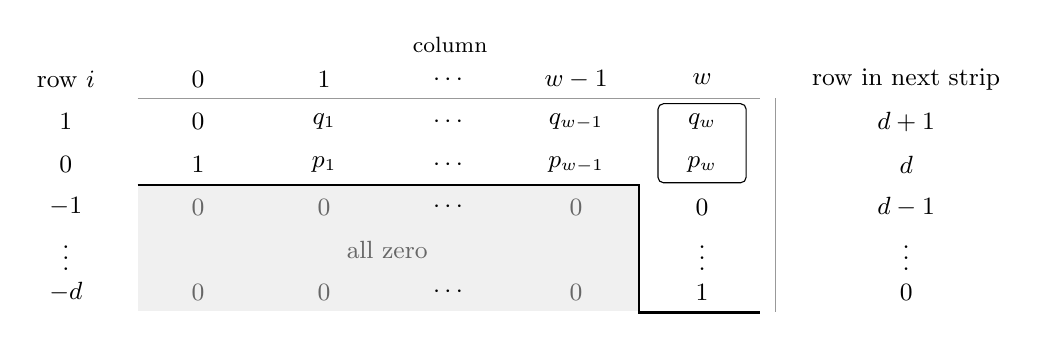
\begin{tikzpicture}[x=16mm,y=5.4mm,font=\small]
  \fill[black!6] (-.48,-3.45) rectangle (3.50,-.48);
  \draw[black!40] (-.48,1.56) -- (4.46,1.56);
  \draw[black!40] (4.58,-3.46) -- (4.58,1.56);
  \node at (-1.05,2) {row $i$};
  \node at (5.62,2) {row in next strip};
  \node[font=\footnotesize] at (2,2.82) {column};
  \foreach \k/\lbl in {0/0,1/1,2/{\cdots},3/{w-1},4/w}
    \node at (\k,2) {$\lbl$};
  \foreach \j/\old/\newrow in {1/1/{d+1},0/0/d,-1/{-1}/{d-1},-2/{\vdots}/{\vdots},-3/{-d}/0} {
    \node at (-1.05,\j) {$\old$};
    \node at (5.62,\j) {$\newrow$};
  }
  \node at (0,0) {$1$}; \node at (0,1) {$0$};
  \foreach \k/\lbl in {1/1,3/{w-1},4/w} {
    \node at (\k,0) {$p_{\lbl}$}; \node at (\k,1) {$q_{\lbl}$};
  }
  \foreach \j in {1,0,-1,-3} \node at (2,\j) {$\cdots$};
  \foreach \k in {0,1,3} {
    \node[text=black!60] at (\k,-1) {$0$};
    \node[text=black!60] at (\k,-3) {$0$};
  }
  \node[text=black!60] at (1.5,-2) {all zero};
  \node at (4,-1) {$0$}; \node at (4,-2) {$\vdots$}; \node at (4,-3) {$1$};
  \draw[line width=.9pt] (-.48,-.48) -- (3.50,-.48) -- (3.50,-3.48) -- (4.46,-3.48);
  \draw[rounded corners=2pt] (3.65,-.43) rectangle (4.35,1.43);
\end{tikzpicture}
\caption{A strip of width $w$ ending in a drop of depth $d$. The heavy line follows the bottom. The new binary word occupies old rows $-d,\ldots,-1$. The boxed entries in old rows $0,1$ become rows $d,d+1$ of the next strip.}\label{fig:shared-column}
\end{figure}

The word at the starting drop begins with \(1,0\), so \((p_0,q_0)=(1,0)\). At each step \(1\le j\le w\), the positive entry \(p_{j-1}\) forces the row-zero digit to be one. Hence \(p_j=1-a p_{j-1}>0\), which forces the row-one digit to be one as well. The two equations become
\[
 p_j=1-a p_{j-1},\qquad q_j=1-p_j-aq_{j-1}=a(p_{j-1}-q_{j-1}).
\]
Two steps in a widest strip give \(q_1=a\) and \(q_2=a(1-2a)\ge0\), so \(a\le1/2\). In fact \(a<1/2\). The roots of \(A\) are algebraic integers because they are roots of the monic integer polynomial \(C\). As a signed elementary symmetric function of these roots, \(a\) is an algebraic integer. A rational algebraic integer is an integer, which excludes \(a=1/2\).

Now take any strip. Induction gives \(1-a\le p_j\le1\) and \(0<q_j\le a\) for \(j\ge1\), since \(p_{j-1}\ge1-a>a\ge q_{j-1}\). Row two receives \(q_j>0\) from below, so its product digit is one and its cofactor entry is at least \(1-q_j-a\ge1-2a>0\). This forces the digit in row three to be one. This proves the assertion through step \(w\).
\end{proof}

\section{Growth across a strip}\label{sec:growth}
The algebraic norm of \(a\) is a nonzero integer. Since \(0<a<1\), some conjugate \(\lambda\) has modulus \(R=|\lambda|>1\). Equation~\eqref{eq:cell} gives \(b_n\in\mathbb Z[a]\) by induction. Apply the embedding \(\sigma:\mathbb Q(a)\to\mathbb C\) that sends \(a\) to \(\lambda\). It fixes the product digits from Lemma~\ref{lem:strip}.

To bound \(R\) from above, take \(D=\{\sigma(b_n):n\in\mathbb Z\}\). For \(b_n>0\) the digit \(c_{n+r}\) is one, so \eqref{eq:cell} gives
\[
 1-\lambda\sigma(b_n)=\sigma(b_{n+r})+\sigma(b_{n+r-m}).
\]
For \(b_n=0\) we can write \(1=1+0\). Thus \(1-\lambda D\subseteq D+D\), and taking diameters gives \(R\,\mathrm{diam}(D)\le2\,\mathrm{diam}(D)\). The set \(D\) is finite and contains \(0,1\), so this gives \(R\le2\).

Fix a strip of width \(w\). At step \(j\) let \(V_j(y)\) encode the cofactor entries in rows zero through three after embedding, with the entry from row \(i\) as the coefficient of \(y^i\). For \(1\le j\le w\) write \(\Delta_j=V_j-V_{j-1}\).

\begin{lemma}[Column differences]\label{lem:growth}
For a strip of width \(w\) preceded by one of width \(v\), there are complex numbers \(\alpha,\beta\) such that, for \(1\le j\le w\),
\begin{equation}\label{eq:growth}
 \Delta_j=(-\lambda)^j(1+y)^{-j}(1+\alpha y^2+\beta y^3)\pmod{y^4},
 \qquad |\alpha|\le R^v,\quad |\beta|\le vR^v .
\end{equation}
\end{lemma}
\begin{proof}
Work modulo \(y^4\), so multiplication by \(y\) shifts an entry up one row. Since row \(-1\) is zero, the four equations at step \(j\) combine to give
\[
 (1+y)V_j+\lambda V_{j-1}=U,\qquad U=1+y+y^2+y^3,\qquad 1\le j\le w.
\]
Subtracting the equations at steps \(j\) and \(j-1\) gives \((1+y)\Delta_j=-\lambda\Delta_{j-1}\) for \(j\ge2\). To include the first step, write its equation as
\[
 (1+y)\Delta_1=U-(1+y+\lambda)V_0=-\lambda\Delta_0 .
\]
This defines the auxiliary initial value \(\Delta_0\) that makes the recurrence hold at the first step. Its relation to the actual difference across the starting drop will depend on the product digits there. Since \(V_0=1\bmod y^2\), the constant and linear coefficients of \(\Delta_0\) are \(1,0\). Write \(\Delta_0=1+\alpha y^2+\beta y^3\). Iteration gives the formula in \eqref{eq:growth} on every strip. In particular the bottom two differences at its last step are \((-\lambda)^w\) and \(-w(-\lambda)^w\), independently of \(\alpha,\beta\).

Let \(v\) be the width of the preceding strip and \(d\) the depth of the drop between them. Use the new row labels on the right of Figure~\ref{fig:shared-column}. The old steps \(v-1,v\) are now columns \(-1,0\). Let \(C_0(y)\) record the four product digits in column zero. Substituting its cell equation \((1+y)V_0+\lambda V_{-1}=C_0\) in the definition of \(\Delta_0\) gives
\[
 \Delta_0=(V_0-V_{-1})+(C_0-U)/\lambda \pmod{y^4}.
\]
In new rows \(d\le i<4\), the old strip supplies a product digit one at its final step. The correction vanishes there, and the old difference passes up by \(d\) rows. Below row \(d\), column \(-1\) is zero and column zero contains the new binary word. A one in the word forces a product digit one and has corrected difference \(1\). A zero has corrected difference \(0\) or \(-1/\lambda\), according to its product digit.

Old row \(i\) becomes new row \(i+d\) at the drop. The coefficients \(\alpha,\beta\) occupy new rows two and three, respectively. Since \(d\ge2\), the only old differences that can reach them are those in the two boxed rows of Figure~\ref{fig:shared-column}. Each entry supplied by the new word has modulus at most one. Thus
\[
\begin{array}{c|cc}
 \text{Drop depth }d & \text{Row two} & \text{Row three}\\ \hline
 2 & \alpha=(-\lambda)^v & \beta=-v(-\lambda)^v\\
 3 & |\alpha|\le1 & \beta=(-\lambda)^v\\
 \ge4 & |\alpha|\le1 & |\beta|\le1
\end{array}
\]
Since \(v\ge1\) and \(R>1\), all three cases give the bounds in \eqref{eq:growth}.
\end{proof}

\section{A Fourier bound for column differences}\label{sec:filter}
At the end of a widest strip of width \(k\), the bottom difference has modulus \(R^k\). For \(R\) close to one this alone gives little growth. The next three rows involve the linear, quadratic, and cubic coefficients of \((1+y)^{-k}\). We will compare their contributions with a bound from the entire product. In fixed coordinates write
\[
 b^\Delta_{i,j}=\sigma(b_{i,j})-\sigma(b_{i,j-1}),\qquad
 c^\Delta_{i,j}=c_{i,j}-c_{i,j-1}.
\]
These arrays are bounded, and \(|c^\Delta_{i,j}|\le1\). Let \(y\) shift entries up one row and \(z\) shift them right one column. Subtracting the cell equations gives
\[
 F*b^\Delta=c^\Delta,\qquad F(y,z)=1+y+\lambda z,
\]
where \(*\) denotes convolution. A polynomial \(P(y)\) combines differences in neighboring rows. To bound \(P*b^\Delta\) it suffices to find \(K=P/F\) with absolutely summable Fourier coefficients \(\widehat K\). The identity \(KF=P\) will then express each filtered entry as a weighted sum of product-digit differences.

Put \(x=R^2\). To choose \(P\), first locate the zeros of \(F\) on the torus \(|y|=|z|=1\). For a fixed \(y\), the zero \(z=-(1+y)/\lambda\) lies on the unit circle precisely when \(|1+y|=R\). The polynomial
\[
 Q(y)=(1+y)^2-xy
\]
detects this condition, since \(Q(y)/y=|1+y|^2-x\). Indeed, \(|Q|=\big||1+y|-R\big|(|1+y|+R)\le |F|(2+R)\) on the torus. Hence \(|Q^2/F|\le(2+R)|Q|\) wherever \(F\ne0\), and the quotient extends continuously by zero at every zero of \(F\).

The coefficients of \((1+y)^{-k}\) alternate. Replacing \(y\) by \(-y\) makes them positive. The cubic \((1+y)Q(-y)\) also has nonnegative coefficients for \(x\ge1\). Its square provides the factor \(Q^2\) needed at the zeros of \(F\). Thus take
\begin{equation}\label{eq:filter}
 P(y)=\big((1-y)Q(y)\big)^2,\qquad
 P(-y)=\big(1+(x-1)y+(x-1)y^2+y^3\big)^2 .
\end{equation}

\begin{proposition}[Fourier bound]\label{prop:kernel}
Let \(1\le|\lambda|=R\le2\), \(F(y,z)=1+y+\lambda z\), and \(P\) be as in \eqref{eq:filter} with \(x=R^2\). The continuous extension \(K\) of \(P/F\) to the torus satisfies
\[
 \sum_{n,s\in\mathbb Z}|\widehat K(n,s)|<25R^3.
\]
\end{proposition}

Appendix~\ref{app:fourier} proves Proposition~\ref{prop:kernel}. To apply it, observe that \(KF=P\) holds on the entire torus, including the zeros of \(F\). Taking Fourier coefficients gives \(\widehat K*F=P\). Proposition~\ref{prop:kernel} gives \(\widehat K\in\ell^1(\mathbb Z^2)\). Since \(F\) has finite support and \(b^\Delta\) is bounded, we may associate the convolutions. Using \(F*b^\Delta=c^\Delta\) and \(|c^\Delta_{i,j}|\le1\) gives
\begin{equation}\label{eq:bound}
 \big|(P*b^\Delta)_{i,j}\big|=\big|(\widehat K*c^\Delta)_{i,j}\big|\le\sum_{n,s}|\widehat K(n,s)|<25R^3
 \qquad (i,j\in\mathbb Z).
\end{equation}
In particular, this bound is independent of the strip width \(k\), whereas the differences at the last column contain the factor \((-\lambda)^k\) from \eqref{eq:growth}.

\section{Excluding a widest strip}\label{sec:end}
\begin{proof}[Proof of Theorem~\ref{thm:main}]
Assume \(0<a<1\) after the normalization of Section~\ref{sec:strip}. Choose a widest strip and write \(k\) for its width. Lemma~\ref{lem:strip} gives \(k\ge5\). Its predecessor has width at most \(k\), so the constants in Lemma~\ref{lem:growth} satisfy \(|\alpha|\le R^k\) and \(|\beta|\le kR^k\).

Translate the array so the chosen strip starts at \((0,0)\). The global bound \eqref{eq:bound} holds in these coordinates, and \eqref{eq:growth} gives the first four differences at step \(k\). Put \(t=x-1\) and denote by \(A_k,B_k,L_k\) the coefficients of \(y,y^2,y^3\) in \(P(-y)(1-y)^{-k}\). Changing the signs back and multiplying by \(1+\alpha y^2+\beta y^3\) shows that the contributions from rows \(i\ge0\) to filtered rows one, two and three are \((-\lambda)^k\) times
\begin{equation}\label{eq:responses}
 -A_k,\qquad B_k+\alpha,\qquad -L_k-A_k\alpha+\beta .
\end{equation}
Here \(A_k=k+2t\). We need lower bounds for \(B_k,L_k\) valid for all \(k\ge5\). Expanding \eqref{eq:filter} at width five gives
\[
 B_5=14x+(t-1)^2,\qquad L_5=(36+6t)x+(t-1)^2 .
\]
Each additional step multiplies the series by \((1-y)^{-1}\), so \(B_{k+1}-B_k=A_{k+1}>0\) and \(L_{k+1}-L_k=B_{k+1}\). Consequently
\begin{equation}\label{eq:lower}
 B_k/x\ge14,\qquad L_k/x\ge36+6t+14(k-5).
\end{equation}

The full convolution also sees the rows below zero. At the last column they contain the newly exposed word \(\eta_i\) (\(i<0\)), extended by zeros below its bottom. Its entries are the actual differences there, since the preceding column was zero below row zero. In particular \(\eta_{-1}=0\) by Lemma~\ref{lem:strip}. Writing \(P_n=[y^n]P(y)\), the boundary contribution in output row \(i=1,2,3\) is
\[
 E_i=\sum_{n=i+2}^6P_n\eta_{i-n},\qquad
 (P_3,P_4,P_5,P_6)=\big(-2(1+t^2),\,t^2+2t,\,-2t,\,1\big).
\]
The positive coefficients sum to \(x^2\). The total modulus of the negative ones is at most \(2x^2\) in row one and at most \(2t\le x^2\) once \(P_3\) is omitted. As each \(\eta_{i-n}\) is zero or one, \(|E_1|\le2x^2\) and \(|E_2|,|E_3|\le x^2\).

To compare with \eqref{eq:bound}, divide by \(xR^k\) and set \(u=R^k/x=R^{k-2}>1\). The global bound becomes \(25/(Ru)\le25/u\) and the three boundary bounds become \(2/u,1/u,1/u\). The bounds on the inherited terms give \(|\alpha|/x\le u\) and \(|\beta|/x\le ku\). For example, row two gives \(|B_k+\alpha|/x<26/u\), hence \(B_k/x<u+26/u\). Using \eqref{eq:responses} and \eqref{eq:lower} in all three rows gives
\begin{align}
 (A_k/x)u &<27, \label{eq:row1}\\
 14\le B_k/x &<u+26/u, \label{eq:row2}\\
 36+6t+14(k-5)\le L_k/x &<(2k+2t)u+26/u. \label{eq:row3}
\end{align}
The first two rows confine \(u\) to a short interval. Since \(x\le4\), we have \(A_k/x=2+(k-2)/x\ge 11/4\), so \eqref{eq:row1} gives \(u<10\). On the interval \([26/10,10]\) the convex function \(u+26/u\) has the same value \(10+26/10<14\) at both endpoints. This entire interval is excluded by \eqref{eq:row2}. Hence \(1<u<26/10\).

Write \((2k+2t)u=10u+2(k-5+t)u\) in \eqref{eq:row3} to separate the contribution at the minimum width from the terms involving \(k-5\) and \(t\). On the interval just obtained,
\[
 36-(10u+26/u)=(u-1)(26/u-10)>0 .
\]
Also \(u<3\), so the rest of the upper bound in \eqref{eq:row3} satisfies \(2(k-5+t)u\le6(k-5+t)\). Adding gives \(L_k/x<36+6t+6(k-5)\), contrary to \eqref{eq:lower}. Thus \(a=1\), and the induction in \eqref{eq:cell} makes \(B\) binary.
\end{proof}

\smallskip\noindent\textit{Verification.} The Lean formalization of Theorem~\ref{thm:main}, including Proposition~\ref{prop:kernel}, uses mathlib and is available on GitHub at \href{https://github.com/esonde/unfair-polynomials-conjecture}{\texttt{esonde/unfair-polynomials-conjecture}}.

\appendix
\section{Proof of the Fourier bound}\label{app:fourier}

We prove Proposition~\ref{prop:kernel}. With \(x=|\lambda|^2=R^2\), the kernel from Section~\ref{sec:filter} is
\[
 K(y,z)=\frac{(1-y)^2\big((1+y)^2-xy\big)^2}{1+y+\lambda z}
\]
on the unit torus, with its continuous extension at the zeros of the denominator. Our goal is to bound the sum of the absolute values of its Fourier coefficients by \(25R^3\). Expanding first in \(z\) gives a geometric series for each fixed \(y\). We then use Parseval's identity in the remaining variable to estimate all the coefficients together.

\subsection*{Expansion in the column variable}
Rotating \(z\) changes only the phases of the Fourier coefficients, so we may set \(\lambda=R\). Write \(y=T^2\) with \(T=e^{i\theta}\) and set
\[
 b=2\cos\theta,\qquad h=b^2,\qquad \omega=4-h .
\]
The substitution doubles row frequencies and preserves the sum of absolute coefficients. Since \(1+T^2=Tb\), \(Q(T^2)=T^2(h-x)\), and \((1-T^2)^2=-T^2\omega\), the kernel becomes
\[
 K(T^2,z)=-T^5\omega\,\frac{(h-x)^2}{b+Rz/T}.
\]
For fixed \(\theta\), expand the quotient in \(z/T\) when \(|b|>R\) and in its reciprocal when \(|b|<R\). The respective coefficients, extended by zero off their branches, are
\[
 g_j(b)=(h-x)^2\frac{(-R)^j}{b^{j+1}}\quad (|b|>R),\qquad
 g_{-j-1}(b)=(h-x)^2\frac{(-b)^j}{R^{j+1}}\quad (|b|<R),
 \qquad j\ge0.
\]
At \(|b|=R\), the extended kernel vanishes for all \(z\). Thus the coefficient of \(z^s\) is \(-T^{5-s}f_s(\theta)\), where \(f_s(\theta)=\omega g_s(b)\). An original row frequency \(n\) becomes \(2n\) under \(y=T^2\). Removing the monomial \(T^{5-s}\) then gives the angular frequency \(p=2n+s-5\) of \(f_s\). By Fubini,
\(\widehat K(n,s)=-\widehat f_s(2n+s-5)\).

Pair the columns \(s=j\) and \(s=-j-1\), assigning both the index \(\ell=|s+1/2|=j+1/2\). The formula for \(g_s\) gives \(f_s(\theta+\pi)=(-1)^{s+1}f_s(\theta)\), so \(\widehat f_s(p)\) can be nonzero only for \(p\equiv s+1\bmod 2\). Thus \(p=2n+s-5\) runs through every frequency that can contribute in column \(s\), and the two columns in a pair have opposite parities. In particular \(\sum_{n,s}|\widehat K(n,s)|=\sum_{s,p}|\widehat f_s(p)|\).

\subsection*{Moments of the column coefficients}
To sum the absolute values over both indices we will use weighted Cauchy--Schwarz. The weight in the column index involves \(\ell\) and \(\ell^3\). In the angular frequency \(p\), a weight of \(p^2\) corresponds by Parseval to one derivative of \(f_s\). The following three moments of \(g_s\) supply these terms.

\begin{lemma}[Column moments]\label{lem:moments}
Put \(\ell_s=|s+1/2|\) and \(M(h)=(h+x)(h-x)^2/2\). For \(b^2=h\ne x\) the functions \(g_s\) above satisfy
\[
\begin{aligned}
 \sum_s\ell_s g_s(b)^2 &= M(h),\\
 \sum_s\ell_s(\ell_s^2-\tfrac14)g_s(b)^2 &= 3hx(h+x),\\
 \sum_s\ell_s|\partial_b g_s(b)|^2 &= \tfrac32(3h^2+x^2).
\end{aligned}
\]
\end{lemma}
\begin{proof}
Take \(v\) near \(b\) on the same branch. Put \(u=bv\) and \(d_b=b^2-x\). The two geometric branches give
\[
 \sum_s\ell_s g_s(b)g_s(v)=d_b^2d_v^2 H(u),\qquad
 H(u)=
 \begin{cases}
 u^{-1}\sum_{j\ge0}(j+\tfrac12)(x/u)^j,& |b|,|v|>R,\\[2pt]
 x^{-1}\sum_{j\ge0}(j+\tfrac12)(u/x)^j,& |b|,|v|<R.
 \end{cases}
\]
Using \(\sum_{j\ge0}(j+\tfrac12)q^j=(1+q)/(2(1-q)^2)\), both branches reduce to
\(H(u)=(u+x)/(2(u-x)^2)\). On compact subsets of either branch the ratio is bounded in modulus by some \(\rho<1\). Derivatives introduce only polynomial factors in \(j\), so we may differentiate the series term by term.

Setting \(v=b\) gives the first identity. In \(H(u)\) the term indexed by \(s\) is a multiple of \(u^{-s-1}\). Applying \(H\mapsto(u^2H')'\) multiplies that term by \(s(s+1)=\ell_s^2-1/4\). Evaluating at \(u=h\) gives the second identity, since \((h-x)^4(u^2H')'|_{u=h}=3hx(h+x)\).

For the derivative moment, use \(d_b d_v=(u-x)^2-x(b-v)^2\) to write
\[
 d_b^2d_v^2H(u)=M(u)-x(u+x)(b-v)^2+x^2(b-v)^4H(u).
\]
Taking \(\partial_b\partial_v\) on the diagonal gives \(M'(h)+hM''(h)+2x(h+x)=\tfrac32(3h^2+x^2)\), proving the third identity.
\end{proof}

\subsection*{Summing the Fourier coefficients}
\begin{proof}[Proof of Proposition~\ref{prop:kernel}]
For \(s=j,-j-1\) write \(\ell=j+1/2\). By the parity relation above, at most one column of the pair contributes at each angular frequency \(p\). Give that term weight \(\ell(\ell^2+16+p^2)\). For fixed \(\ell\), the sum of \((\ell^2+16+p^2)^{-1}\) over \(p\) is of order \(1/\ell\). The additional factor \(\ell\) makes the reciprocal weights summable over \(j\). At low frequencies the constant \(16=4^2\) supplies a uniform lower bound for the denominator. Applying Cauchy--Schwarz on finite sets of indices and then taking limits gives
\[
 \sum_{s,p}|\widehat f_s(p)|\le\sqrt{SE},\qquad
 S=\sum_{j\ge0}\sum_{p\in\mathbb Z}\frac{1}{\ell(\ell^2+16+p^2)} .
\]
With \(\langle\,\cdot\,\rangle\) denoting normalized angular average, Parseval gives the weighted sum
\[
 E=\sum_{j\ge0}\sum_{s\in\{j,-j-1\}}
       \ell\left\langle(\ell^2+16)|f_s|^2+|\partial_\theta f_s|^2\right\rangle .
\]
The double zero in \(g_s\) at \(|b|=R\) makes each zero extension continuously differentiable, as required for the derivative term.

To bound \(S\), compare its inner sum with an integral. On the unit interval centered at \(p\) the average of \(q^2\) is \(p^2+1/12\). Jensen's inequality for the reciprocal therefore gives
\[
 S\le\sum_{j\ge0}\frac1\ell\int_{\mathbb R}
 \frac{dq}{q^2+\ell^2+16-1/12}
 =\pi\sum_{j\ge0}\frac1{\ell\sqrt{\ell^2+16-1/12}}.
\]
Put \(a_\ell=\sqrt{\ell^2+16-1/12}\). Then \(a_\ell\ge\max(4,\ell)\). Use \(4\) for \(j=0,1,2\), and \(\ell\) thereafter. Since \(1/(j+1/2)^2\le 1/j-1/(j+1)\), the tail telescopes and
\[
 S/\pi\le \tfrac14(2+2/3+2/5)+\tfrac13=\tfrac{11}{10}.
\]

To compute \(E\), integrate the derivative of \(f_s=\omega g_s\) by parts over one period. For \(g=g_s(b)\) this gives
\[
 \big\langle|\partial_\theta(\omega g)|^2\big\rangle
 =\big\langle \omega^2|\partial_\theta g|^2-\omega\omega''g^2\big\rangle .
\]
Here \((\partial_\theta b)^2=\omega\) and \(-\omega\omega''=2\omega(\omega-h)\). The switching angles \(|b|=R\) form a finite set. Away from them Lemma~\ref{lem:moments} identifies each sum in the energy. The sums of squares may be integrated term by term by monotone convergence. The series for the signed term is absolutely integrable, since \(|\omega\omega''|\sum_s\ell_s g_s^2=|\omega\omega''|M(h)\) almost everywhere. Thus, with \(M=M(h)\),
\[
 E=\Big\langle \omega^2\big(\tfrac{65}{4}M+3hx(h+x)\big)
      +2\omega(\omega-h)M+\tfrac32\omega^3(3h^2+x^2)\Big\rangle .
\]
Substituting \(\omega=4-h\) leaves a polynomial of degree five in \(h\). Its angular average sends \(h^n\) to \(\binom{2n}{n}\), the constant term of \((T+T^{-1})^{2n}\). Thus the six monomials have averages \(1,2,6,20,70,252\), giving
\[
 4E=211x^3+38x^2-107x+542\le684x^3 .
\]
Indeed, \(x\ge1\) gives \(38x^2\le38x^3\) and \(542-107x\le435\le435x^3\).
Combining the two bounds gives \(SE\le(11\pi/10)\,171R^6<625R^6\), since \(\pi<22/7\).
\end{proof}

\begin{thebibliography}{1}
\bibitem{dvorsky}
A. Dvorsky, \emph{The unfair 0--1 polynomial problem and high-degree trinomials}, 2026, \href{https://arxiv.org/abs/2608.19173v2}{arXiv:2608.19173v2}.
\bibitem{dvorsky-finite}
A. Dvorsky, \emph{Trinomials of the type $1+ax^2+x^k$ in the unfair $0$--$1$ polynomial problem}, manuscript, version~4, 4 August 2026.
\bibitem{ghidelli}
L. Ghidelli, \emph{Progress on the unfair 0--1-polynomials conjecture using linear recurrences and numerical analysis}, 2022, \href{https://arxiv.org/abs/2209.09843}{arXiv:2209.09843}.
\bibitem{hare}
K. G. Hare, \emph{Computational progress on the unfair 0--1 polynomial conjecture}, Experimental Mathematics, published online 15 July 2025, \href{https://doi.org/10.1080/10586458.2025.2527786}{doi:10.1080/10586458.2025.2527786}.
\bibitem{hasanbegovic}
E. Hasanbegovi\'c, \emph{Structural results on the unfair 0--1 polynomial conjecture}, 2026, \href{https://arxiv.org/abs/2611.14596}{arXiv:2611.14596}.
\end{thebibliography}
\end{document}
